% +--------------------------------------------------------------------+
% | Sample Chapter 3
% +--------------------------------------------------------------------+

\cleardoublepage

% +--------------------------------------------------------------------+
% | Replace "This is Chapter 3" below with the title of your chapter.
% | LaTeX will automatically number the chapters.
% +--------------------------------------------------------------------+

\chapter{Diseño de la aplicación}
\label{makereference3}

\section{Stakeholders}
\label{makereference3.1}
En este apartado hablaremos de aquellos grupos que tengan un cierto interés sobre nuestra aplicación. Cuando se planteó
la idea de este proyecto observamos que, como su nombre indica, su dominio es el ocio, siendo en este caso en particular el mundo del cine.
\\
La aplicación surge de la necesidad de aquellas personas de querer ver una película acompañados, ya sea por amigos o por usuarios que tengan un gusto similar, 
siendo la afinidad de las personas a cierta película una faceta importante de nuestra aplicación a la hora de tomar una decisión. Con esto queremos reflejar que 
cualquier persona que posea un cierto grado de cinefilia podrá pertenecer al grupo de stakeholders.
\\
También podríamos incluir empresas dedicadas al sector de actividades de exhibición cinematográfica en España tales como Cinesa o Yelmo, ya que podríamos incluir 
una forma de redirigir a la compra de entradas para una película en la que el usuario está interesado para una de las dos entidades anteriores.
\newpage 
\section{Escenarios}
\label{makereference3.2}
Antes de decidir como implementaríamos nuestra aplicación decidimos que sería importante establecer una serie
de escenarios en los que podría ser usada. Tras esto pudimos ponernos de acuerdo en que funcionalidades incluiríamos y que 
éstas se ajusten a las necesidades de los usuarios. Además, estos escenarios deberían usar la \textbf{realidad aumentada} para que 
les aporte valor, ya que, como hemos expuesto anteriormente en el capítulo 2, el grueso de nuestra aplicación se centra en esta tecnología.

\paragraph{Escenario 1. Usando la aplicación en casa:\\}
\begin{itemize}
    \item Te apetece ir al cine y encuentras el cartel de una película que te interesa ver en cualquier lado (ordenador, revista, etc.), sacas tu móvil con la aplicación y 
    la escaneas, con la realidad aumentada te saldrán los distintos paneles y botones que te facilitan información sobre la película:
    \begin{enumerate}
        \item Ver el tráiler.
        \item Valoración que tiene en páginas web, como por ejemplo \textbf{IMDB}.
        \item Botón para crear un plan para ir a ver esa película o unirte a uno que uno de tus amigos ya haya creado para esa misma película.
        \item Botón para guardar la película en tu lista de películas guardadas.
    \end{enumerate}
    \item Te apetece ir al cine y has visto varias películas que te interesan, pero no sabes a cuál ir, captas todas ellas con la aplicación 
    y para cada una de ellas tendrás las opciones anteriores más poder añadirlas a un plan ya creado, crear un nuevo plan o guardarlas.
\end{itemize}
\newpage
\paragraph{Escenario 2. Usando la aplicación en la calle.\\}
En este escenario, queremos solucionar el problema que aparece cuando el usuario de la aplicación se encuentra con el cartel de una película y pretende registrarla en su aplicación lo más rápido posible.
Este escenario se produce mayormente cuando el usuario está paseando por la calle, en el metro, en un centro comercial…
\\
El usuario podrá rápidamente escanear el cartel de la película y guardar así ésta en su lista de películas para posteriormente añadirla a un plan o poder ver la información de ésta, además de la opción de poder valorarla.
\\
Este escenario requiere que el usuario guarde rápidamente la película, puesto que el usuario puede tener prisa y simplemente esté pasando cerca de un cartel mientras va a otro sitio.



\section{Requisitos funcionales}
\label{makereference3.3}

\paragraph{\large Planes:\\}

Los planes están compuestos por una película, un usuario creador del plan, y los usuarios que se hayan unido. El plan
es creado debido a la necesidad que tiene un usuario de querer ver una película específica con una serie de usuarios que 
entrarán en el plan por tener interés en ver dicha película debido a su afinidad con la misma.
\\
\textbf{Funciones:}
\begin{enumerate}
    \item \textbf{Crear plan}: para crear un plan un usuario ha tenido que guardar previamente una película tras reconocerla con la cámara y al entrar a la interfaz de la información de dicha película podrá presionar el botón para crear un plan con dicha película.
    \item \textbf{Unirse a un plan}: dependiendo de si el plan es privado o público solo podrán unirse los amigos del usuario creador del plan o cualquiera, al entrar en la interfaz que tiene la información de un plan podremos pulsar un botón para unirnos.
    \item \textbf{Información de un plan}: simplemente con presionar en un plan podremos ver la información del mismo, es decir, la película a ver y los usuarios que se han unido.
\end{enumerate}
\newpage
\paragraph{\large Películas guardadas:\\}

Las películas guardadas son aquellas que el usuario ha decidido guardar para ver su información más tarde o para posteriormente añadirlas a un plan.
\\
\textbf{Funciones:}
\begin{enumerate}
    \item \textbf{Guardar película}: cuando un usuario reconoce una película con la cámara, le aparecerá un botón que le permitirá guardar la película como favorita, para poder ver su información posteriormente o crear un plan con ella.
    \item \textbf{Información de una película}: un usuario puede ver la información de una película que haya guardado con presionar en la misma. Podrá ver una pequeña sinopsis, el género y el director, además de la posibilidad de poder valorarla.
\end{enumerate} 

\section{Sistema de recomendación}
\label{makereference3.5}
Para la implementación de los sistemas de recomendación nos hemos encontrados con tres librerías:
\begin{enumerate}
    \item \textbf{Mahout}: Se trata de una librería bastante compleja, que básicamente abarca la mayoría de necesidades para la implementación del sistema de recomendación.
    \item \textbf{Lenskit}: Es otra librería de java que para la implementación de sistemas de recomendación.
    \item \textbf{LibRec}: Esta está colgada en un repositorio de github, se trata de una librería de terceros.
\end{enumerate}

Al final se ha decantado por \textbf{Mahout}, pues es la librería más conocida de las tres. Además, que aporta una buena documentación, otro motivo es que ofrece clases para la conexión directamente con base de datos y sin tener que leer desde ficheros csv. Por otro lado, en el testeo de librería de \textbf{Lenskit}, cuando se intentaba reproducir el ejemplo que ofrecían, se encontraban que algunas funciones estaban obsoletas y, por tanto, no daban mucha confianza. Por último, \textbf{Mahout} se destaca por minimizar el uso del esfuerzo.

\section{Prototipos}
\label{makereference3.6}

\subsection{ARCore} 
\label{makereference3.6.1} 
\begin{flushleft}
    Al comenzar la fase de desarrollo de proyectos, pensamos que una de las tecnologías que debíamos 
    investigar y probar debía ser \textbf{ARCore}. Esto se debía a que, la empresa detrás de esta 
    tecnología es \textbf{Google} y esto podría significar que tendríamos más material de consulta 
    y ejemplos en comparación con otras tecnologías de fabricantes con menos recursos.
    \textbf{ARCore} se encuentra disponible para \textbf{Java}, \textbf{Unity}, \textbf{Unreal} e \textbf{iOS}. Comenzamos realizando el 
    "Quickstart" para \textbf{Android} y posteriormente para \textbf{Unity}. 
    Tras realizar los proyectos propuestos por \textbf{ARCore}, realizamos algún proyecto propio 
    para comprobar si la herramienta se ajustaba a la idea que teníamos para nuestro futuro proyecto.
    Tras realizar ambos proyectos, concluimos que, aunque \textbf{ARCore} reúne las características 
    necesarias para en un futuro convertirse en una de las tecnologías más importantes en Realidad Aumentada, 
    no íbamos a seleccionarla para nuestro proyecto por las siguientes razones:
    \begin{enumerate}
        \item \textbf{ARCore} dispone de mucha documentación para comenzar a usar la herramienta, pero poca para realizar tareas más complejas
        \item \textbf{ARCore} resulta muy útil para realizar superposiciones de modelos 3D sobre superficies, sin embargo, una de las funcionalidades más importantes que nuestra aplicación requería era la interacción con la realidad aumentada mediante el uso de botones, imágenes y la carga dinámica de elementos para posicionar en la pantalla de Realidad Aumentada e interaccionar con el usuario. En este sentido \textbf{ARCore} no está, por el momento, tan preparada como otras tecnologías.
    \end{enumerate}
    
\end{flushleft}
\subsection{Viro Media} 
\label{makereference3.6.2}
\begin{flushleft}
El objetivo del prototipo realizado con \textbf{Viro Media} es reconocer imágenes almacenadas en el dispositivo para mostrar texto y
 objetos virtuales. Además de probar tecnologías de desarrollo móvil web como en este caso \textbf{React Native}
 para plataformas \textbf{iOS} y \textbf{Android}.
\end{flushleft}
\begin{flushleft}
Comenzamos construyendo una interfaz sencilla con botones que nos redirigen a la escena de Realidad Aumentada.
Para esta interfaz utilizamos \textbf{NativeBase} que es una librería que nos permite
realizar una aplicación con apariencias de tipo \textbf{iOS} o \textbf{Android} según el dispositivo.
\end{flushleft}

\begin{figure}[htb]
    \centering
    \makebox[0pt][c]{%
    \begin{minipage}[b]{0.5\linewidth}
    \centering
      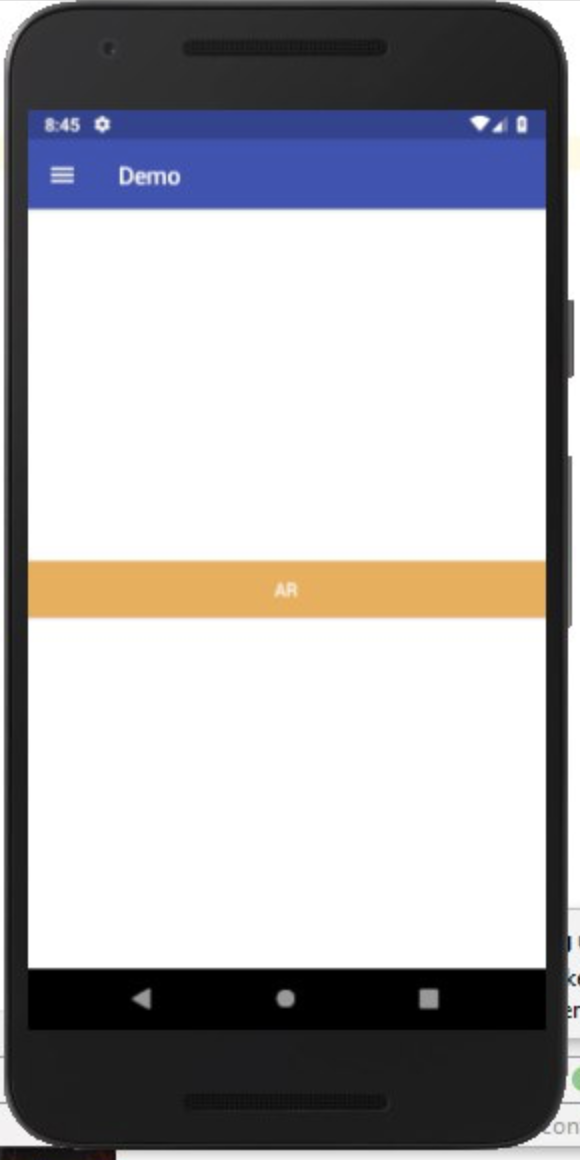
\includegraphics[scale=0.3]{figures/chapter-3/viromedia/android.png}
      \caption{Visualización con NativeBase en Android}
    \label{sva}
    \end{minipage}%
    \hspace{0.3cm}
    \begin{minipage}[b]{0.5\linewidth}
    \centering
     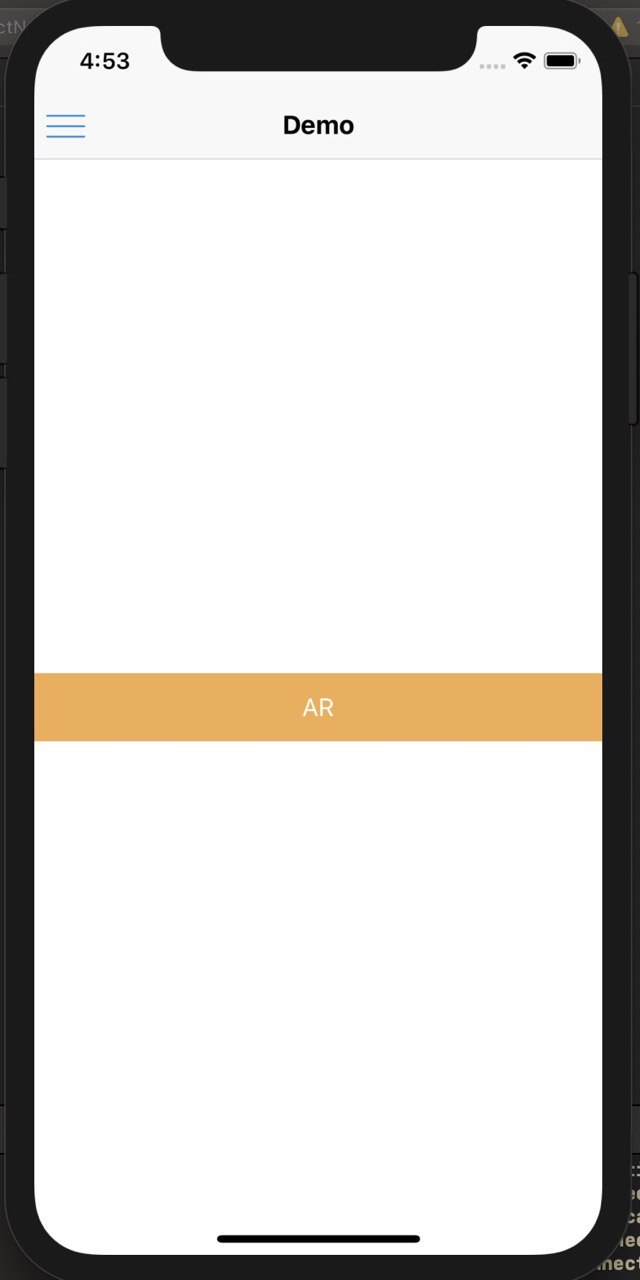
\includegraphics[scale=0.3]{figures/chapter-3/viromedia/ios.jpg}
      \caption{Visualización con NativeBase en iOS}
    \label{svb}
    \end{minipage}%
    }%
\end{figure}

\begin{flushleft}
Para la escena de Realidad Aumentada mostramos texto y al detectar el póster de Pantera Negra,
 reacciona mostrando una animación de dicho súper héroe saliendo del póster.
\end{flushleft}
 
\begin{figure}[H]
    \centering
    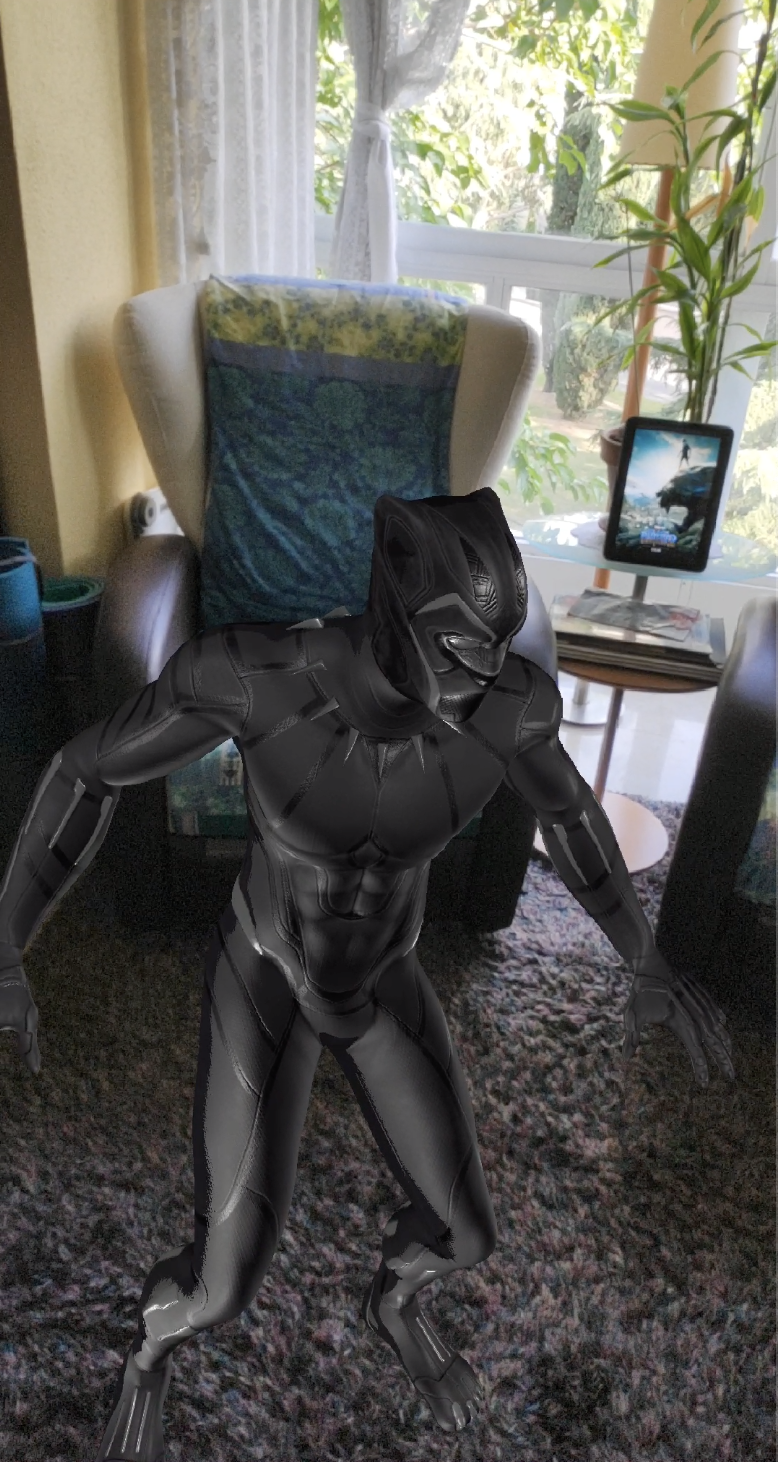
\includegraphics[width=3in]{figures/chapter-3/viromedia/blackpanther.png}
    \caption{Visualización de RA}
\end{figure}

\begin{flushleft}
Una de las ventajas que apreciamos fue la facilidad del lenguaje, en este caso \textbf{Javascript},
 utilizando la popular librería \textbf{ReactJS} y la buena documentación de \textbf{Viro Media}
 que hacían que el proceso de codificación fuera agradable.
\end{flushleft}
\begin{flushleft}
Uno de los problemas que presentaba este prototipo era que las dependencias de \textbf{Viro Media} entraban en conflicto con las de \textbf{NativeBase}
imposibilitándonos la forma de encontrar versiones compatibles. Utilizamos las últimas que, a pesar de lanzar
 advertencias, funcionaba en el ejemplo realizado.
Otro problema fue la compilación de la aplicación, \textbf{Viro Media} tiene una aplicación para probar lo
 que desarrollamos conectándose a nuestro ordenador a través de la red. El problema es
 que algunos recursos, como los iconos que utilizaba \textbf{NativeBase}, no eran descargados, por lo que la
 mejor forma era probar la versión compilada de \textbf{iOS} y \textbf{Android}. La forma de compilar
 la aplicación era un proceso costoso para los ordenadores, lento y con multitud de problemas según
 se ampliaban las librerías que se utilizan.
\end{flushleft}

\begin{flushleft}
La conclusión que obtuvimos de este prototipo fue que \textbf{Viro Media} y \textbf{React Native} son tecnologías muy prometedoras, pero debido a los
 problemas surgidos y a que todas sus versiones no eran estables vimos un claro riesgo para
 nuestro proyecto.
\end{flushleft}

\newpage
\subsection{Vuforia + Android} 
\label{makereference3.6.3} 
 
\begin{flushleft}
En este prototipo utilizamos la librería nativa de \textbf{Vuforia} para \textbf{Android} para 
realizar las pruebas de tecnología de reconocimiento de imágenes tanto en  
local como usando la nube que nos ofrecía \textbf{Vuforia}, para la posterior renderización
de objetos y textos.

Las características tecnológicas de este prototipo son las siguientes:
\end{flushleft}

\begin{enumerate}
    \item La librería de \textbf{Vuforia} para \textbf{Android} está diseñada a muy bajo nivel.
    \item \textbf{Vuforia} para dibujar en 3D usa la librería \textbf{OpenGL}.
    \item \textbf{OpenGL} utiliza una serie de espacios donde se van colocando los elementos: 
    \begin{enumerate}
        \item \textbf{Local space}: Es el espacio local de cada objeto.
        \item \textbf{World space}: Es el mundo donde se encuentran los objetos.
        \item \textbf{View space}: El mundo visto desde la perspectiva de la cámara.
        \item \textbf{Clip space}: Se integra con la pantalla del móvil y, definiendo los límites visibles, se establecen unas coordenadas de rango (-1,-1) - (1,1).
    \end{enumerate}
    \begin{flushleft}
        Las transformaciones de estos espacios se realizan mediante matrices 4x4, 
        en las que la primera fila hace referencia a la coordenada x, la segunda a la coordenada y y la 
        tercera a la coordenada z, mientras que la última columna hace referencia a los desplazamientos 
        de los objetos en esos 3 ejes.
        \end{flushleft}
        

        
            \begin{figure}[H]
                \centering
                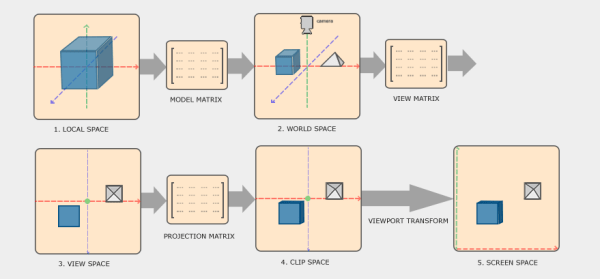
\includegraphics[width=5in]{figures/space-transformation.png}
                \caption{Esquema de los distintos espacios que usa OpenGL}
            \end{figure}

            \begin{figure}[H]
                \centering
                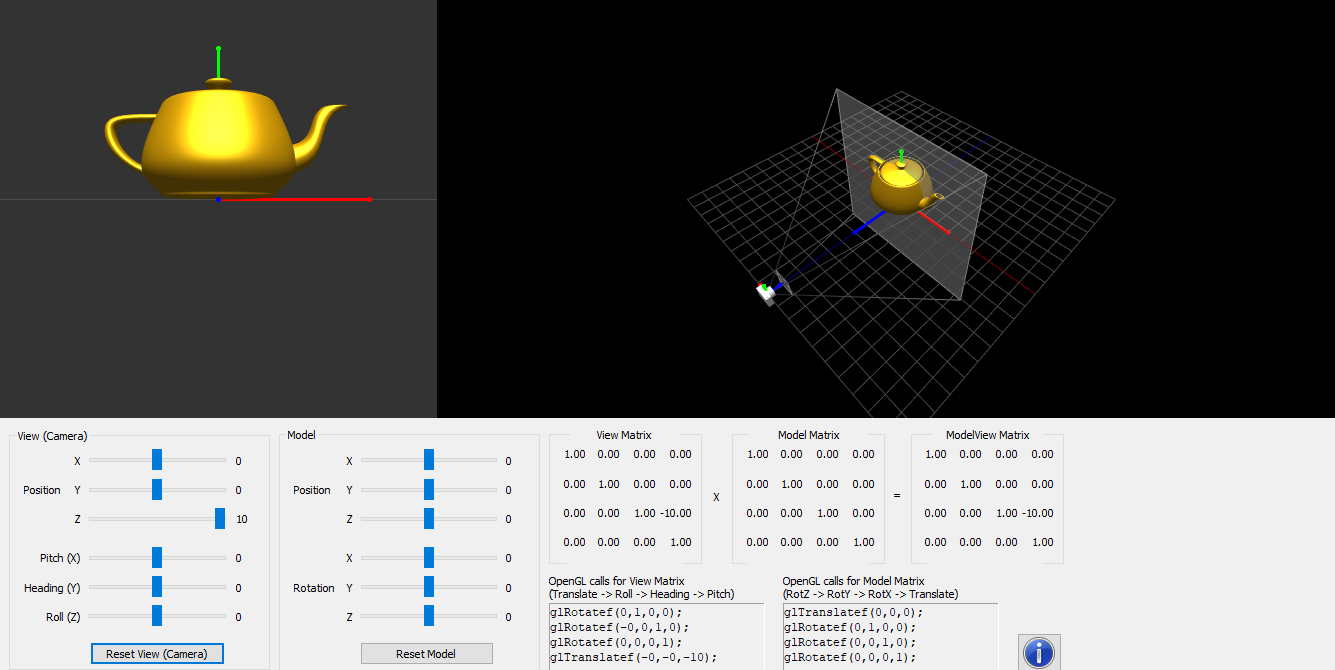
\includegraphics[width=5in]{figures/teapot.png}
                \caption{Ejemplo de un modelo en 3D}
            \end{figure}
    
    \item En \textbf{OpenGL} es necesario escribir código para que las tarjetas gráficas rendericen el modelo 3D,
    el lenguaje que se usa es \textbf{GLSL}. Este código de \textbf{GLSL} se escribe en forma de \textbf{String} y se llama a un método 
    que proporciona \textbf{OpenGL}.
    \begin{figure}[H]
        \centering
        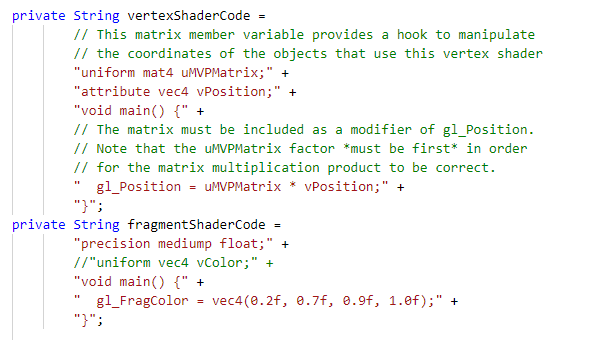
\includegraphics[width=5in]{figures/GLSL.png}
        \caption{Código en GLSL}
    \end{figure}
        
    \item Otro aspecto a tener en cuenta es que \textbf{OpenGL} solo nos ofrece lo básico, no nos ofrece métodos para dibujar 
    directamente objetos, sino que hay que seguir un pipeline de procesos para conseguir dibujar algo.
    \newline
    \begin{flushleft}
    Esto consiste en pasar un \textbf{array} de números (cada tres para definir un punto) 
    a las tarjetas gráficas, establecer triángulos entre los puntos (más arrays de números) 
    definir colores a partir de los puntos (más arrays)..., y con el código del shader, ejecutar 
    estos datos.
    \begin{figure}
        \centering
        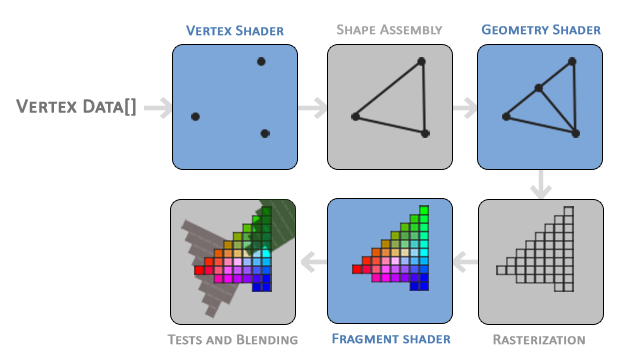
\includegraphics[width=4in]{figures/pipeline.png}
        \caption{Pipeline de la construcción de un modelo}
    \end{figure}
    \end{flushleft}
    \newpage
    \item Por último, como sólo ofrece métodos básicos, no hay métodos de escritura de texto, y la forma que 
    encontramos y que funcione fue usar un bitmap con los caracteres. Rechazamos esto por un principal motivo, para hacer que funciones hay que codificar a muy bajo nivel y 
    nos costaría mucho tiempo y esfuerzo.
    \begin{figure}
        \centering
        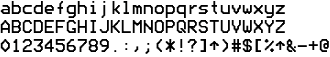
\includegraphics[width=5in]{figures/bitmap-font.png}
        \caption{Mapa de bits de caracteres usado}
    \end{figure}
\end{enumerate}
 

\newpage
\subsection{Vuforia + Unity} 
\label{makereference3.6.4}
\begin{flushleft}
    Para realizar este prototipo utilizamos \textbf{Unity} como herramienta básica para realizar la aplicación y \textbf{Vuforia} para dar soporte a la Realidad Aumentada.
    El prototipo a desarrollar consistió en un modelo 3D de un dragón que aparecía al detectar una imagen que previamente habíamos establecido como ``imagen objetivo''.
\end{flushleft}
    \begin{figure}[H]
        \centering
        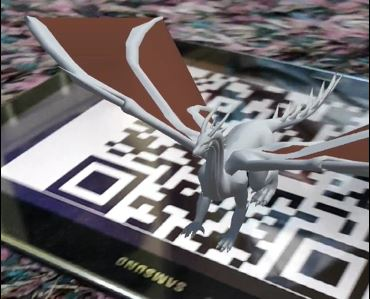
\includegraphics[width=5in]{figures/prototipoUnity.jpg}
        \caption{Modelo en 3D que aparecía al detectar la imagen}
    \end{figure}
\begin{flushleft}
    Pese a que nadie del equipo había utilizado \textbf{Unity} previamente el resultado fue bastante positivo ya que:
    \begin{enumerate}
    \item \textbf{Unity} resultó ser intuitivo y relativamente fácil en cuanto al aprendizaje de las funcionalidades básicas.
    \item \textbf{Vuforia} parecía estar muy probada e incluía de serie muchas funcionalidades.
    \item \textbf{Vuforia} tenía la opción de utilizar un \textbf{Cloud} para almacenar las imágenes objetivo.
    \end{enumerate}
\end{flushleft}

\subsection{Vuforia + Unity + Android} 
\label{makereference3.6.5}
\begin{flushleft}
Una vez realizado el prototipo en \textbf{Vuforia} con \textbf{Unity} comenzamos a investigar cómo realizar el resto de la aplicación que no requería de Realidad Aumentada.
\break
Hasta este momento teníamos claro que \textbf{Vuforia} con \textbf{Unity} era la mejor combinación para realizar la parte de Realidad Aumentada, sin embargo, \textbf{Unity} no era igual de intuitivo ni eficaz a la hora de realizar tareas propias de una aplicación "normal", como el desarrollo de interfaces o la lógica.
\break
Por este motivo intentamos buscar la opción de realizar una aplicación en la que la Realidad Aumentada estuviese diseñada en \textbf{Unity} con \textbf{Vuforia} y el resto de la aplicación en Android.
\end{flushleft}
\begin{figure}[H]
        \centering
        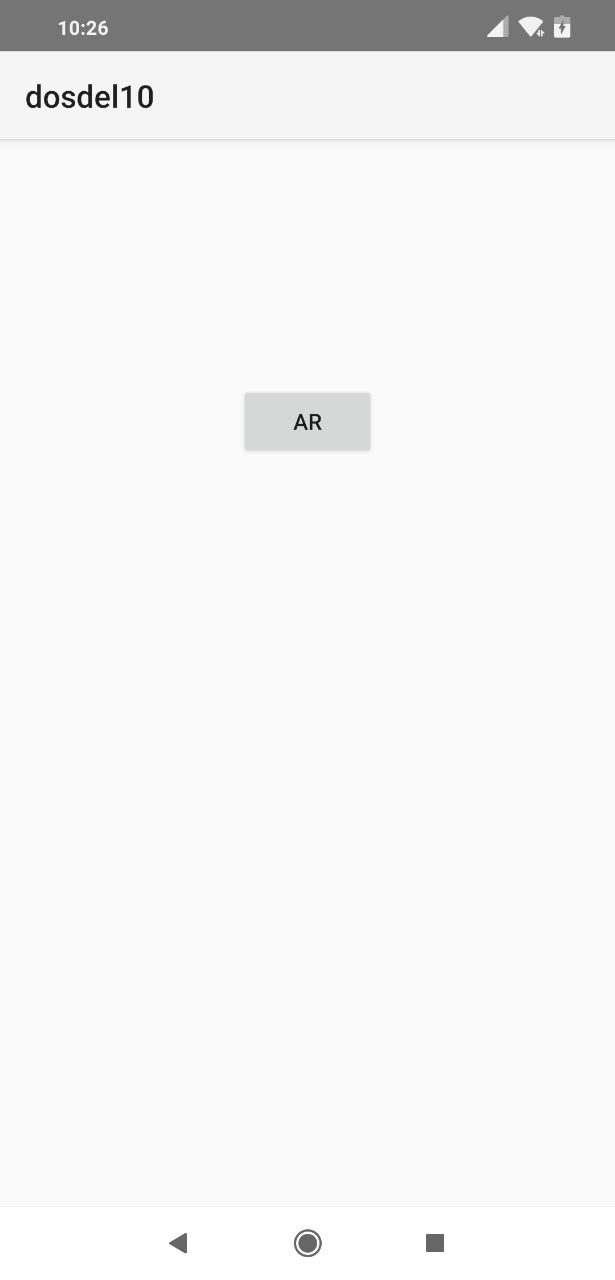
\includegraphics[width=1in]{figures/androidUnityVuforia.jpg}
        \caption{Botón que comunicaba Android con Unity}
\end{figure}
\begin{flushleft}
    Finalmente conseguimos tener ambos proyectos independientes, la Realidad Aumentada se desarrollaba en \textbf{Unity} con \textbf{Vuforia} y se exportaba a un proyecto Android donde se encontraba el resto de la aplicación.
    Esto nos permitía realizar la Realidad Aumentada con la herramienta que tras las primeras tomas de contacto habíamos comprobado que era la mejor (\textbf{Unity} con \textbf{Vuforia}) y del mismo modo realizar el resto de la aplicación con la mejor herramienta para esta parte (AndroidStudio).
\end{flushleft}
\begin{flushleft}
    Tras realizar este prototipo, consideramos que estas herramientas podrían ser las que usásemos en la aplicación final puesto que:
    \begin{enumerate}
    \item Como ya habíamos descubierto en el prototipo anterior, \textbf{Unity} era una herramienta muy completa y junto con \textbf{Vuforia} nos proporcionaban todas las herramientas necesarias para cumplir con los casos de uso de Realidad Aumentada que teníamos en mente.
    \item Al haber encontrado la forma de combinar \textbf{Unity + Android} no teníamos que renunciar a ninguna de las dos herramientas. Lo que nos permitía explotar las cosas buenas de ambas herramientas.
    \item La comunicación entre \textbf{Unity} y Android era relativamente sencilla pese a ser dos proyectos distintos.
    \end{enumerate}
\end{flushleft}

\newpage
\subsection{Server en Spring} 
\label{makereference3.6.6}

\begin{flushleft}
    Para la realización de la parte backend de la aplicación decidimos
    incorporar la tecnología de \textbf{Spring} para codificar un \textbf{servicio web REST} en \textbf{Java}
    y el acceso a datos mediante \textbf{MySQL}.
\break
\break
    Para el prototipo seguimos el siguiente tutorial: 
\newline
Cómo crear un microservicio o servicio web REST con Spring Boot\cite{tutorialspring}
\break
    que consistía en 3 partes bien definidas para la creación de dicho \textbf{servicio web REST} para la gestión de una entidad de contactos muy simple, se puede observar su estructura
    en la figura 3.6.
    \begin{figure}[H]
        \centering
        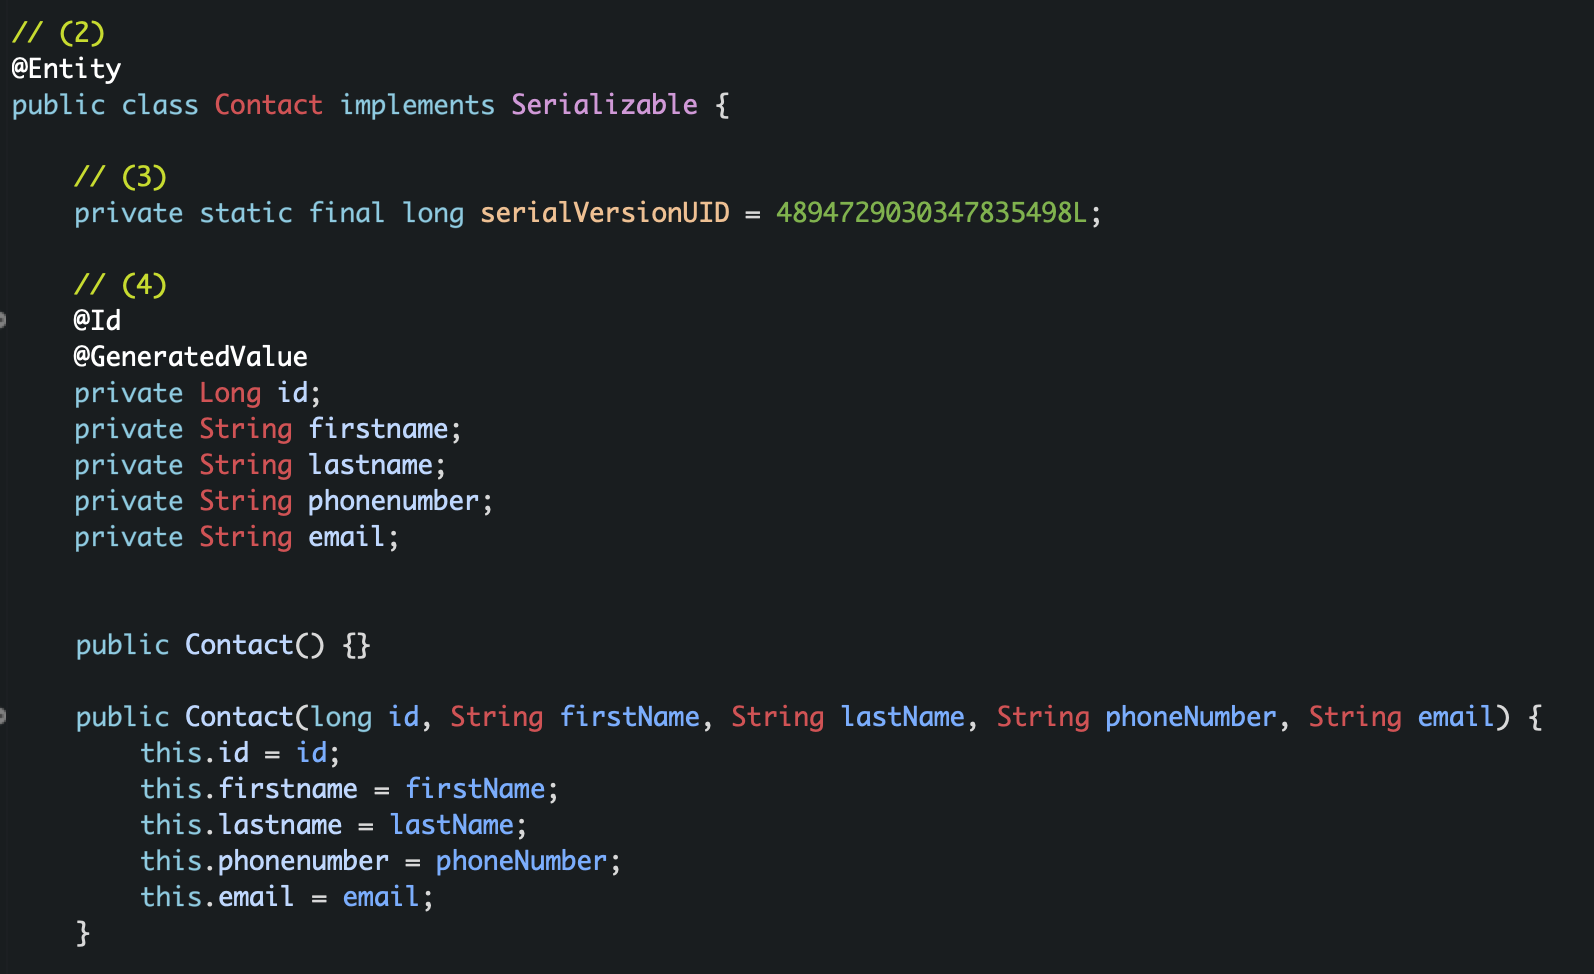
\includegraphics[width=6in]{figures/ContactsEntity.png}
        \caption{Entidad de Contactos}
    \end{figure}
\break
\break
    También se investigaron distintas formas de realizar el acceso a la base de datos desde el servidor, pero finalmente nos decantamos por usar la
    clase \textbf{JPARepository} o \textbf{CRUDRepository}, las cuales nos ofrecen ya implementados los métodos típicos de las operaciones \textbf{CRUD}, además de la opción 
    de poder crear nuestros propios métodos.
\end{flushleft}

\begin{flushleft}
    Para poder probar las distintas peticiones de tipo \textbf{POST} y \textbf{GET}, que realizamos en local, usamos la herramienta 
    \textbf{Postman}, ver figura 3.7.
    \begin{figure}[H]
        \centering
        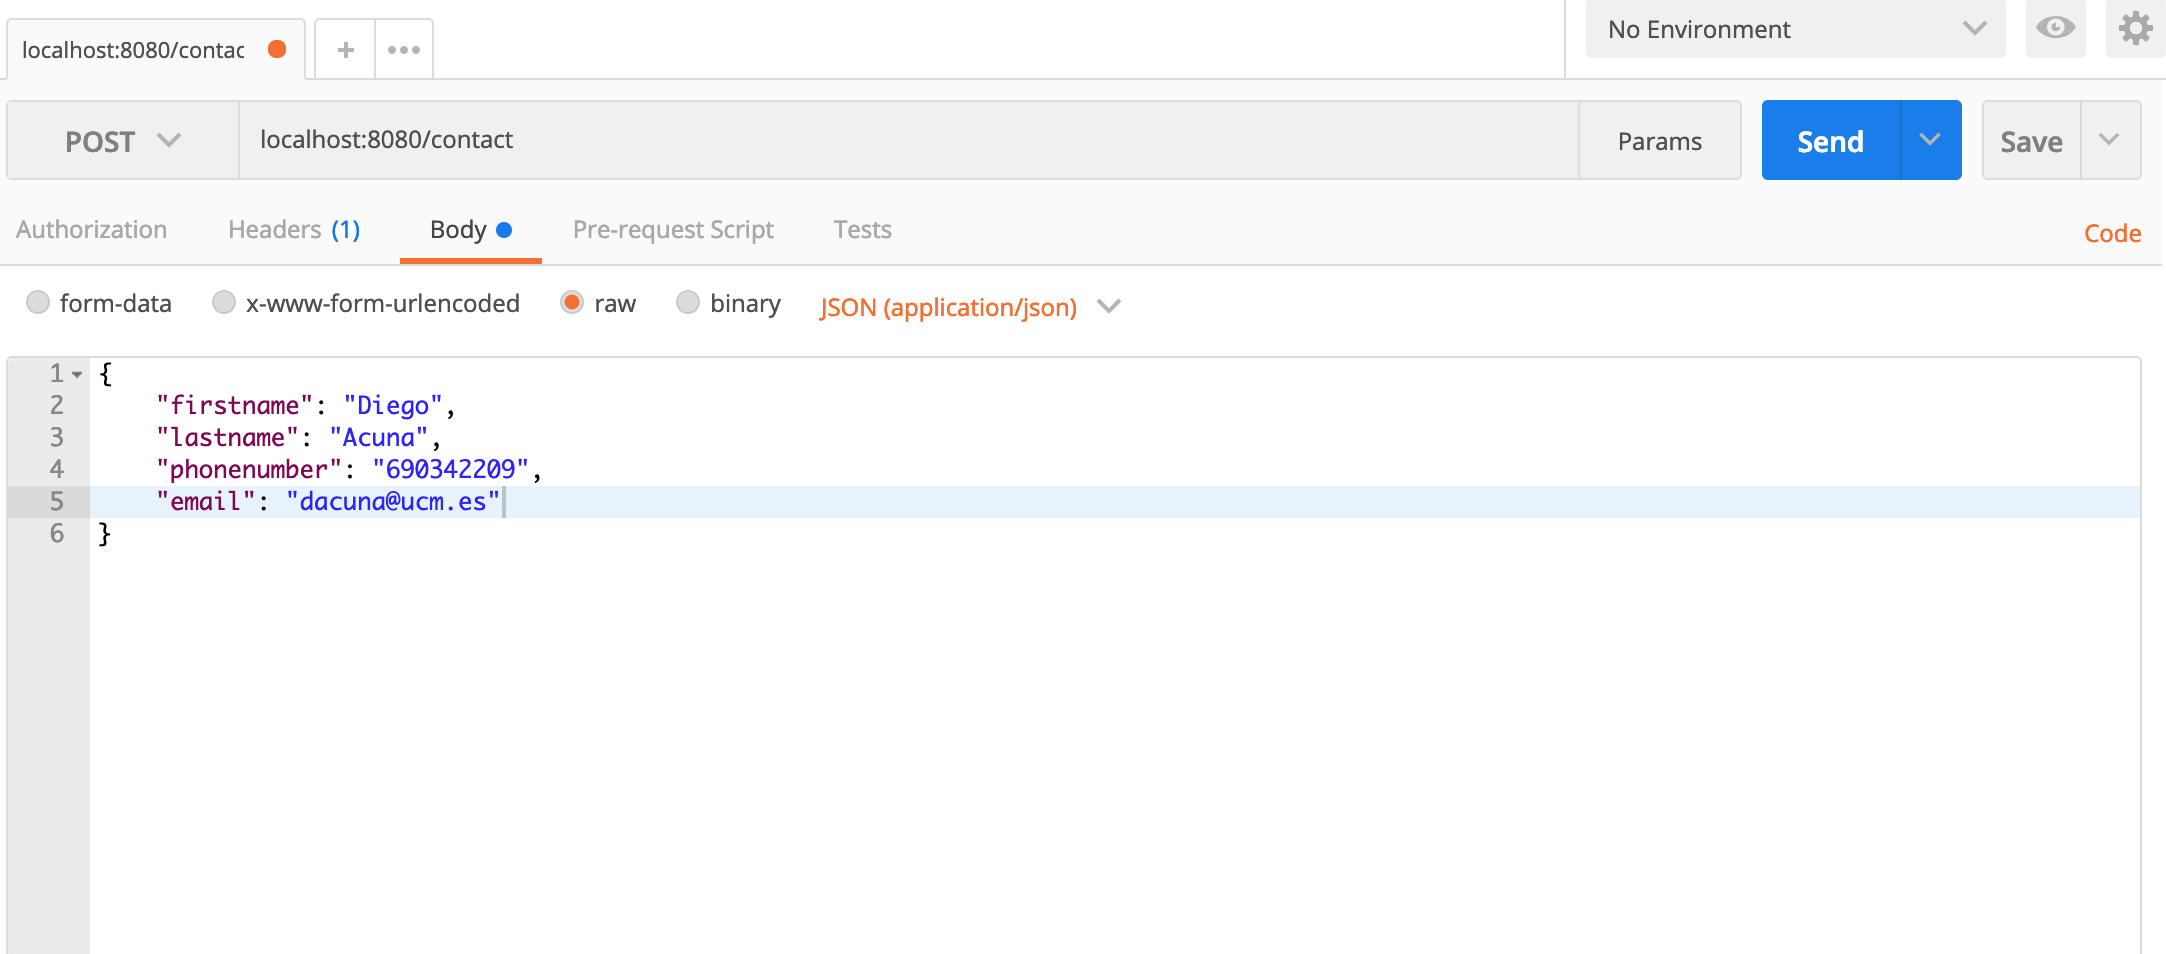
\includegraphics[width=6in]{figures/Postman.png}
        \caption{Postman}
    \end{figure}
    Para este prototipo decidimos usar \textbf{MySQL} como sistema de gestión de bases de datos relacional, aunque
    a la hora de probar a levantar nuestro servidor de prueba tuvimos que rehacer este prototipo, además de adaptarlo para 
    que gestionara entidades de películas, y que usara \textbf{PostgreSQL}, además de cambiar una serie de anotaciones y limpiar 
    el archivo \textbf{pom.xml} de líneas de código innecesarias, ver figura 3.8, que es el que contiene las dependencias de nuestro proyecto.
    \begin{figure}[H]
        \centering
        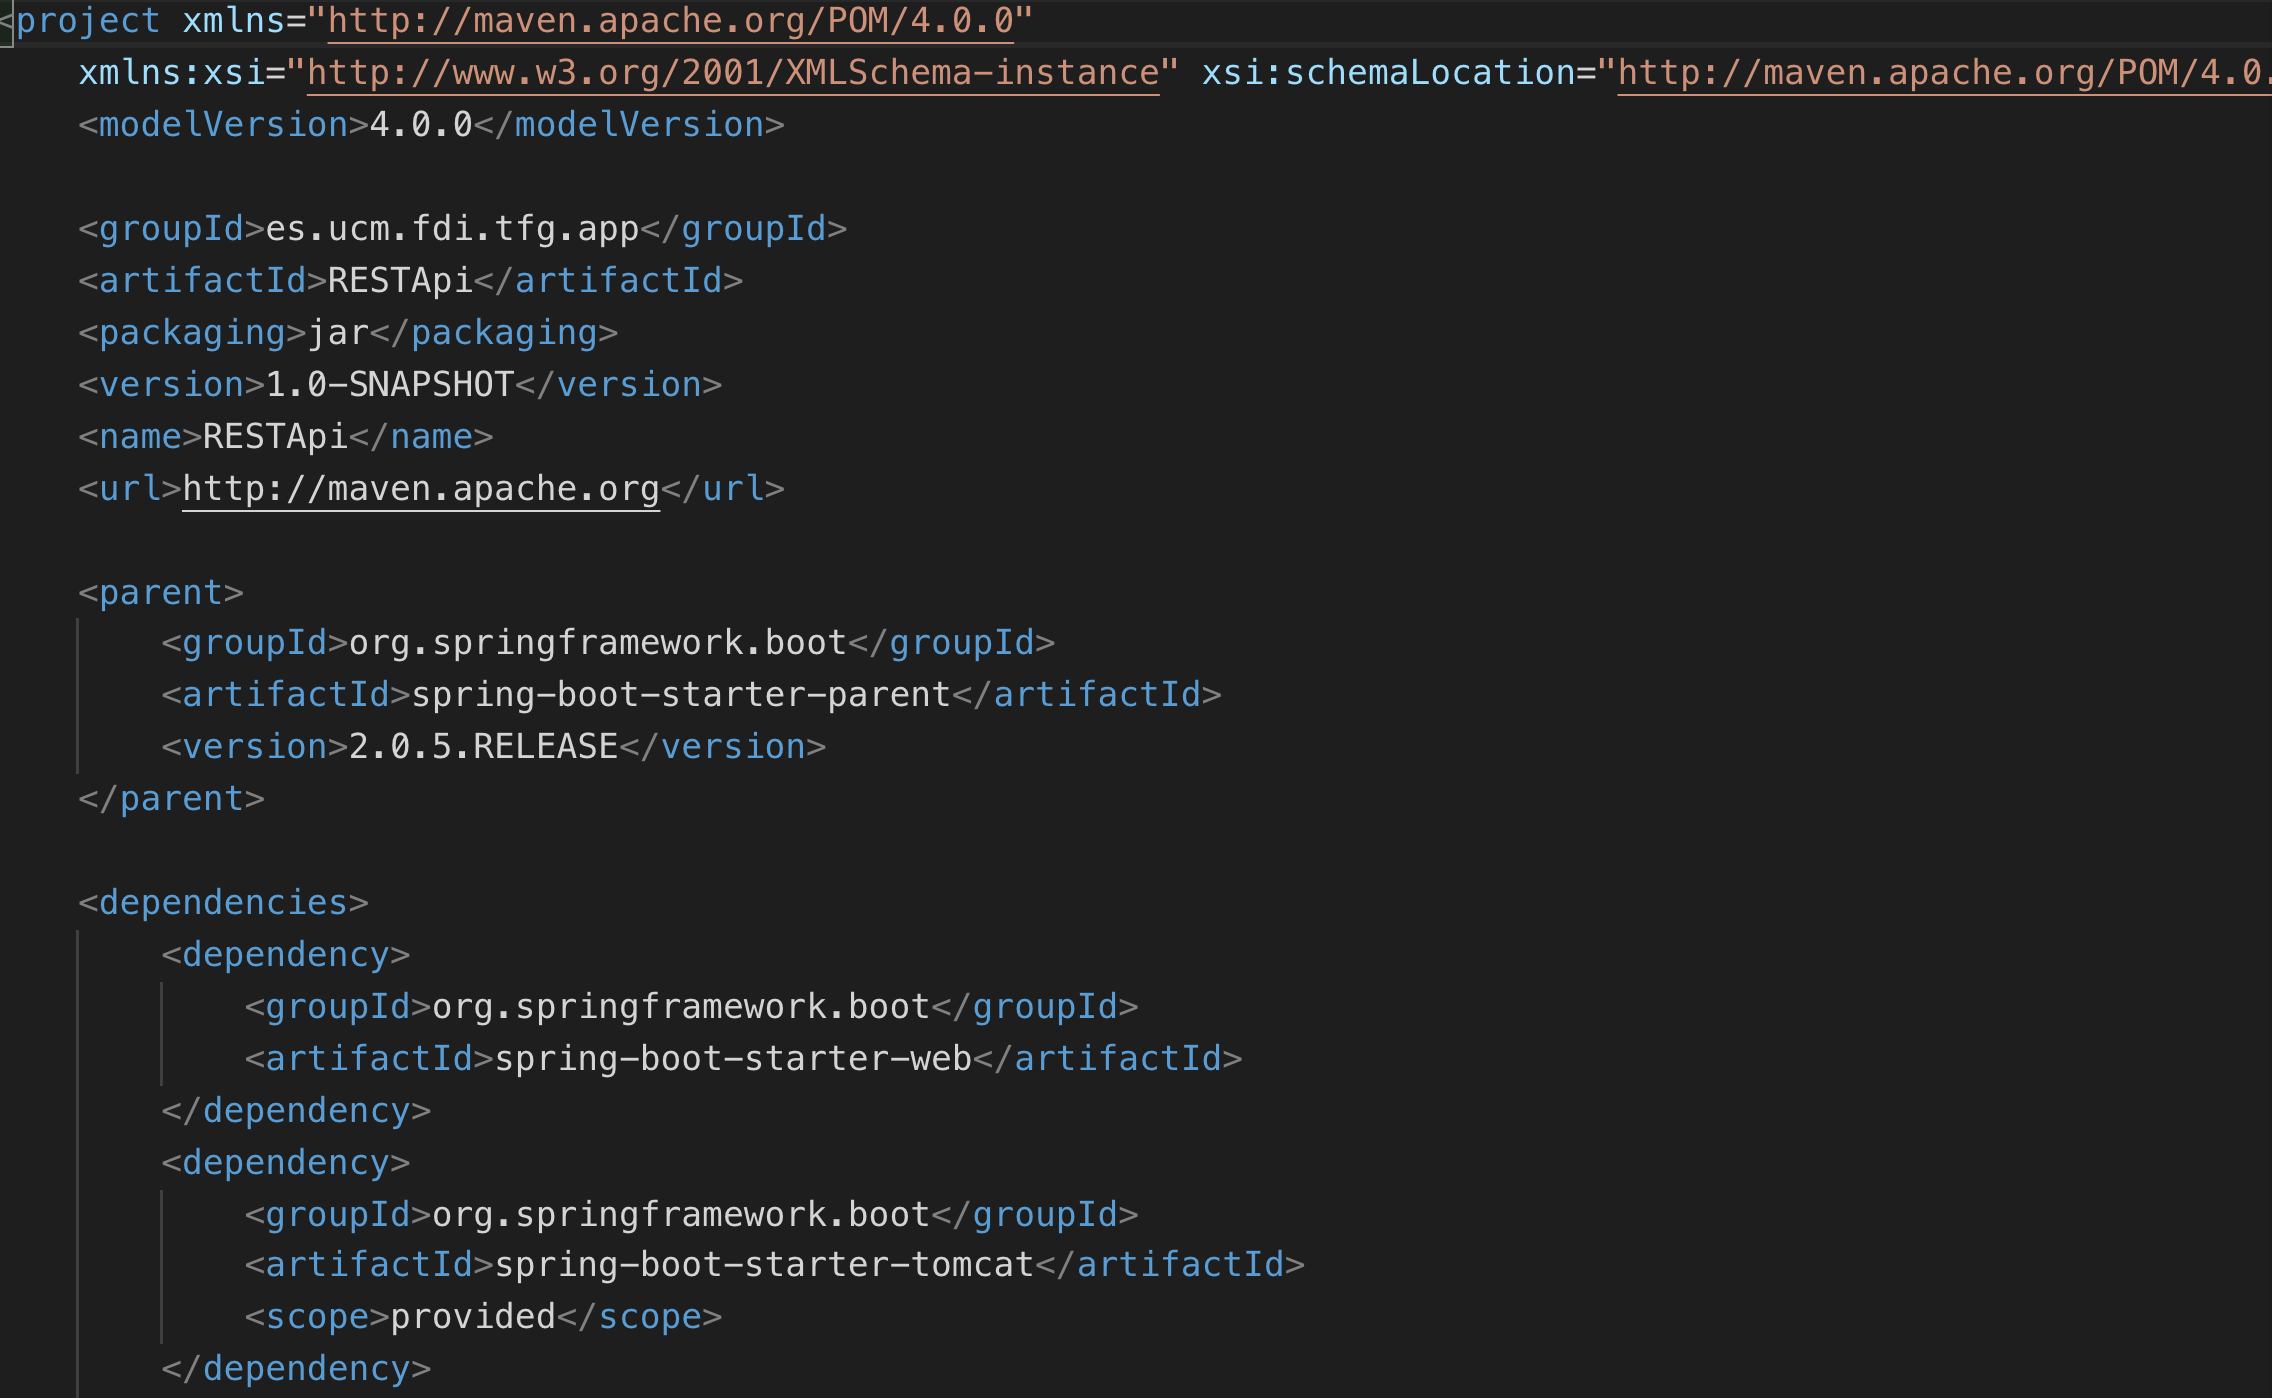
\includegraphics[width=6in]{figures/PomXML.png}
        \caption{Archivo pom.xml}
    \end{figure}
\end{flushleft}
\section{Interfaz de usuario}
\label{makereference3.4}

A continuación, mostraremos las distintas interfaces de usuario de nuestra aplicación y la evolución que han ido sufriendo.
\subsection{Interfaz de lista de planes}
\label{makereference3.4.1}
El objetivo de esta vista es el de mostrar los planes públicos que existen, indicando con una imagen de fondo la película para la que se creó el plan, el usuario
que creó dicho plan y los usuarios que se han unido. La primera vista que realizamos fue la siguiente
\begin{figure}[H]
    \centering
    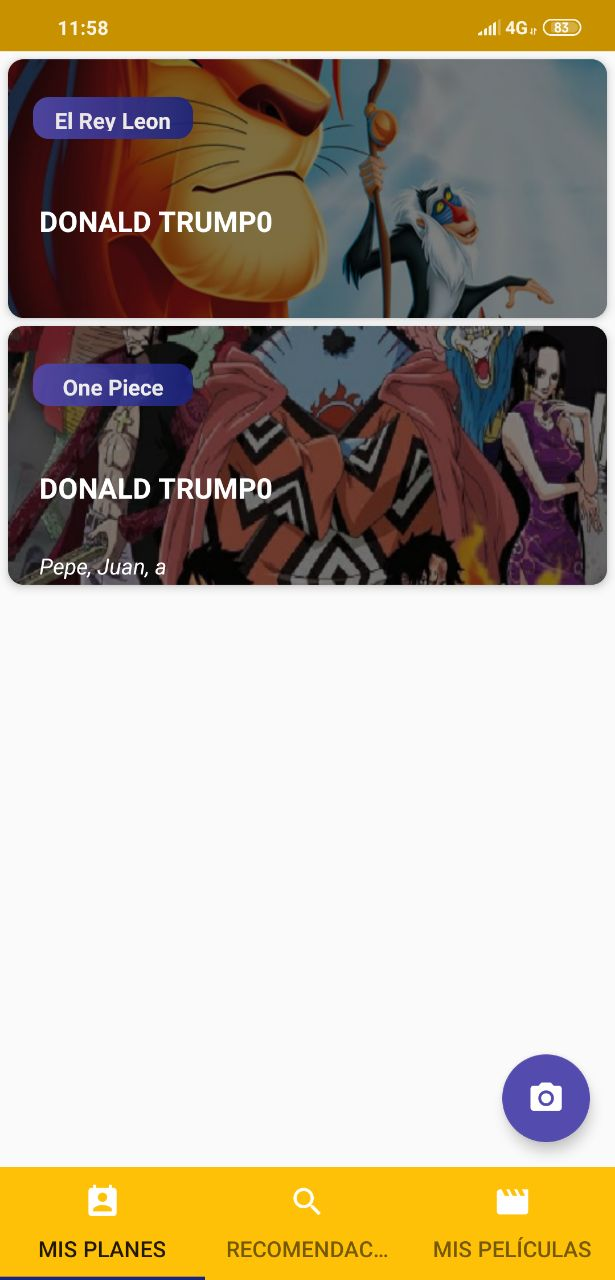
\includegraphics[width=3in]{figures/PlansList1.jpg}
    \caption{Lista de planes, primera versión}
\end{figure}
Podemos observar como cada elemento representa un plan, con el fondo siendo el cartel de la película, el título de la película en la esquina superior izquierda,
debajo el nombre del usuario que lo ha creado junto con las personas que se han unido al plan.
\\
Tras mostrarla en una de las reuniones con los directores de nuestro TFG, nos sugirieron cambiarla debido a que no reflejaba correctamente lo que era, es decir, 
cada plan no otorgaba la información suficiente a un usuario para que éste supiera que era un plan en sí. Por lo que posteriormente decidimos cambiar la vista
para mostrar al usuario la estructura de un plan correctamente y así ofrecerle una mejor experiencia de usuario. 
\\
La siguiente figura muestra la segunda versión de nuestra lista de planes: 
\begin{figure}[H]
    \centering
    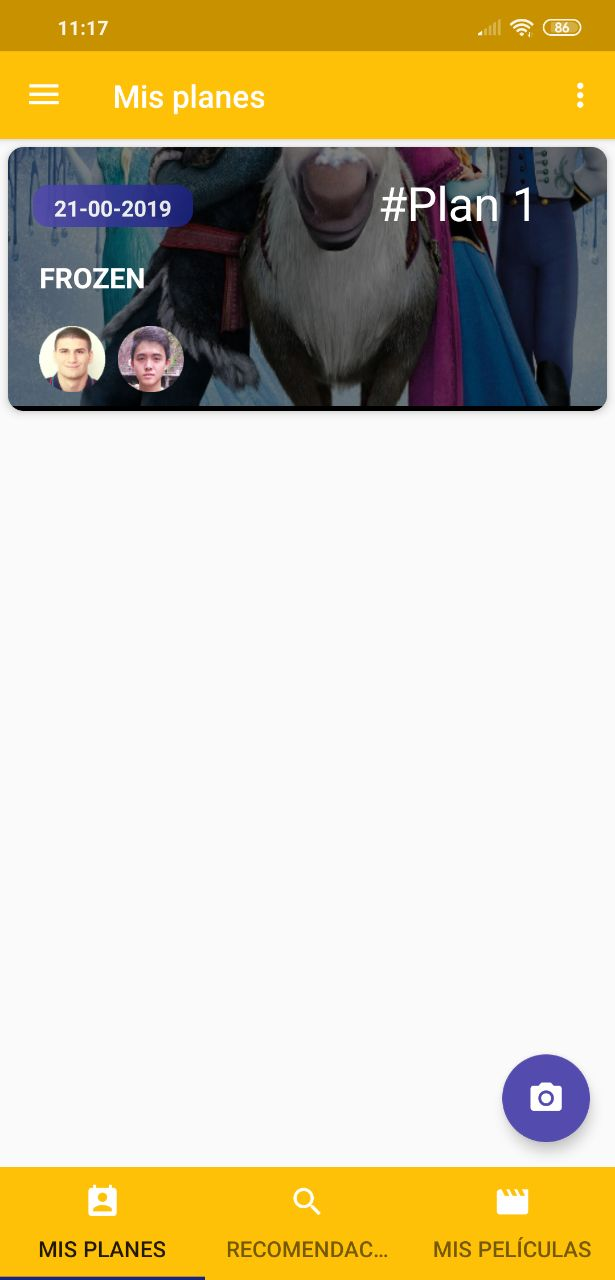
\includegraphics[width=3in]{figures/planslist2.jpg}
    \caption{Lista de planes, segunda versión}
\end{figure}
Podemos observar como ahora aparece la fecha para la que es el plan en la parte superior izquierda, justo debajo el título de la película que se quiere ver, arriba a la derecha el número del plan, algo simple pero que nos indica
claramente lo que representa este elemento.
El cambio más significativo es que, ahora en la parte inferior aparecen las fotos de los usuarios que se han unido al plan.
\subsection{Interfaz de lista de películas guardadas}
\label{makereference3.4.2}
Para mostrar las películas guardadas decidimos usar un grid que muestre solamente los carteles de las películas, es una interfaz simple pero muy visual, para acceder a la información
de cada película simplemente debemos pulsar en uno de los carteles.
\begin{figure}[H]
    \centering
    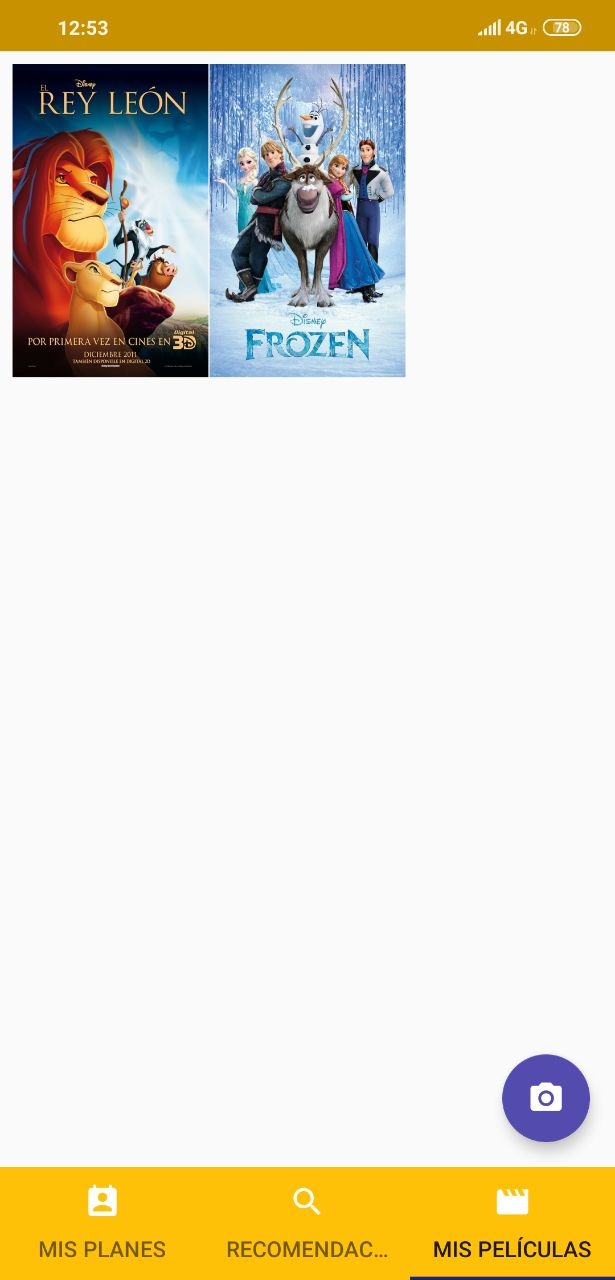
\includegraphics[height=5in]{figures/FilmsList.jpg}
    \caption{Lista de películas guardadas}
\end{figure}
En la figura 3.3 podemos observar que el usuario solo ha guardado 2 películas, si se guardaran más irían apareciendo al lado de las que ya están o pasarían debajo en cuanto una 
fila tuviera 3 elementos, elegimos este tamaño para que pudieran verse correctamente los carteles y los títulos de las películas.
\subsection{Interfaz principal}
\label{makereference3.4.3}
En la figura 3.3 también vemos como es la interfaz principal, con una barra en la parte inferior para movernos por las 3 secciones de nuestra aplicación: \textbf{mis planes}, \textbf{recomendaciones}, \textbf{mis películas}.
Cada sección incluye un icono para apoyar a la representación.
Además, encontramos un botón con un símbolo de una cámara en todas las secciones que nos permitirá acceder a la parte de \textbf{Realidad Aumentada}

\subsection{Interfaz de realidad aumentada al reconocer una película}
\label{makereference3.4.4}
En esta interfaz destacamos los distintos componentes que aparecen al usar la cámara de nuestro teléfono y reconocer el cartel de una película.
Lo primero que podemos observar al entrar a la interfaz de realidad aumentada es una especie de simulación de un escáner que se superpone a lo que vemos con la
cámara del teléfono, incitando así al usuario a reconocer algo con la cámara, esto lo podemos ver en la figura 3.4.

\begin{figure}[H]
    \centering
    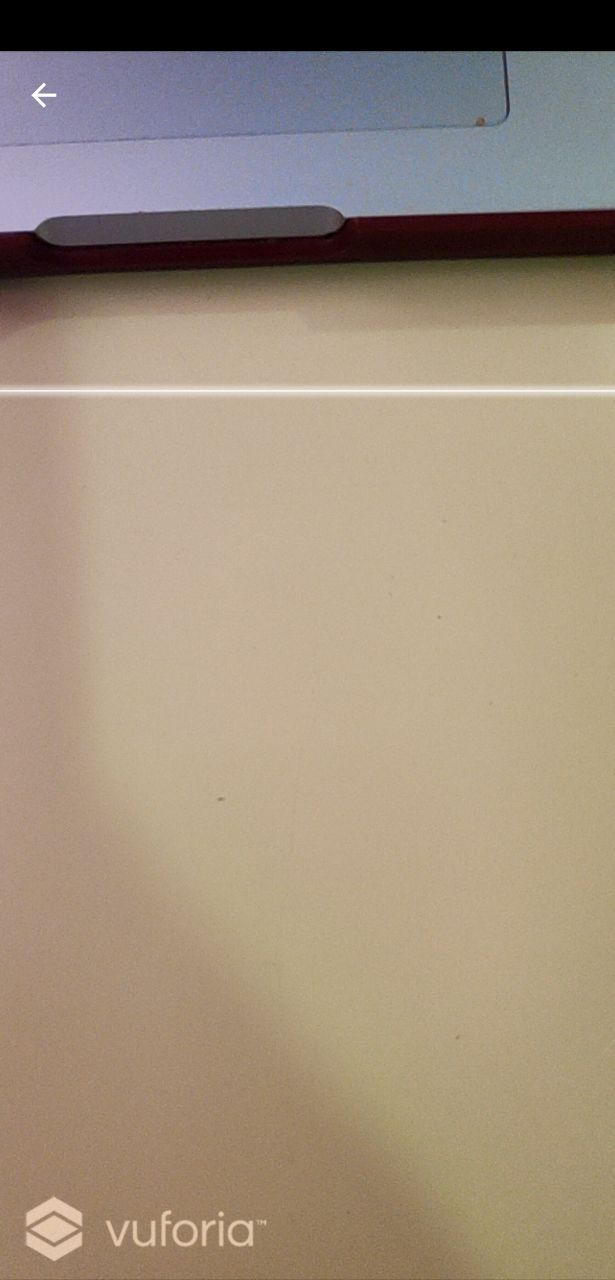
\includegraphics[width=3in]{figures/escaner.jpg}
    \caption{Escáner}
\end{figure}

Cuando reconocemos un cartel, sobre la imagen de la película nos aparecerá en la parte superior una valoración numérica de la película, la cual la hemos 
sacado de \textbf{IMDB}. justo en el medio de la imagen encontramos el icono típico de \textbf{Youtube} que, al pulsarlo, nos abrirá nuestra aplicación de \textbf{Youtube} para que
el usuario pueda ver el tráiler de esta película. En la esquina inferior derecha encontramos otro icono que al ser pulsado lo que hará será desplegar una serie de botones con distinta funcionalidad,
uno de ellos nos redirige a la información de la película en \textbf{IMDB}, que sería el icono representado por una letra \textbf{i}, el otro botón representado por una mano con un pulgar hacia arriba nos permitirá
guardar la película en nuestra lista de películas guardadas, para posteriormente acceder a su información, valorarla o crear un plan con ella. Todo esto lo podemos observar en la figura 3.5 y 3.6.
\begin{figure}[H]
    \centering
    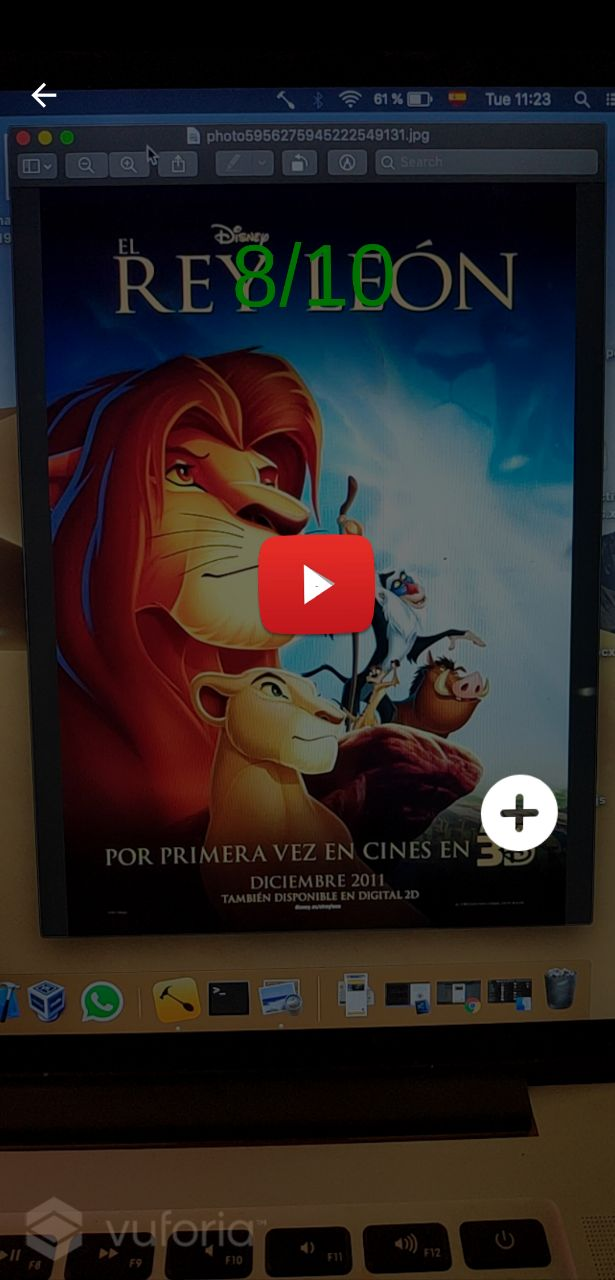
\includegraphics[width=3in]{figures/filmrecognized1.jpg}
    \caption{Realidad aumentada tras reconocer una película}
\end{figure}
\begin{figure}[H]
    \centering
    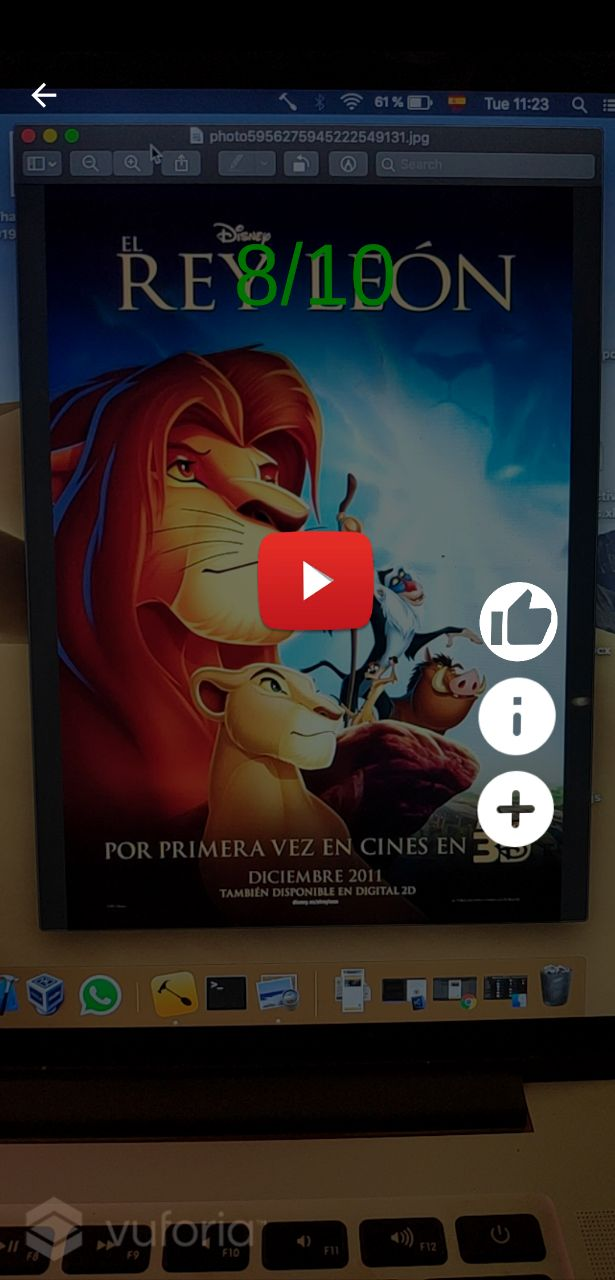
\includegraphics[width=3in]{figures/filmrecognized2.jpg}
    \caption{Realidad aumentada tras reconocer una película}
\end{figure}

\newpage
\subsection{Interfaz de realidad aumentada al reconocer a un usuario}
\label{makereference3.4.5}
\begin{flushleft}
Cuando reconocemos a un usuario de la aplicación con la cámara de nuestro dispositivo se pueden dar dos casos,
 que sea amigo del usuario que lo está reconociendo o que todavía no lo sea.
\end{flushleft}
\begin{flushleft}
Si no es un amigo aparecerá una interfaz para añadir al usuario como amigo, mientras que si es un amigo 
aparecerá una interfaz distinta en donde el usuario puede incorporarse a los planes de su amigo.
\end{flushleft}
\subsection{Interfaz de realidad aumentada al reconocer a un usuario que no es amigo}
\label{makereference3.4.5.1}
\begin{flushleft}
Se trata de una interfaz sencilla en donde al usuario que enfoca se le proporciona el nombre del usuario al
 que está enfocando (siempre que el usuario enfocado esté registrado) junto a un botón de añadir amigo.
\end{flushleft}
\subsection{Interfaz de realidad aumentada al reconocer a un usuario que sí es amigo}
\label{makereference3.4.5.2}
\begin{flushleft}
Esta interfaz que aparece al enfocar con la cámara a un usuario que es amigo del que enfoca, es una interfaz
 más compleja que la anteriormente descrita.
\end{flushleft}
\begin{flushleft}
Cuando un usuario enfoca a otro que es amigo, se proporciona la opción de incorporarse a uno de los planes del
 amigo. Para ello, se le muestra una interfaz con los tres planes que según nuestro algoritmo de recomendación
  más pueden interesarle de los que su amigo tiene.
\end{flushleft}
\begin{flushleft}
La interfaz proporciona la imagen de las películas de los tres planes, además, mediante una interfaz dinámica 
podemos movernos de un plan a otro, de esta forma podemos ver quien hay en el plan junto a la puntuación que 
nuestro sistema de recomendación calcula que le gusta a cada participante el plan.
\end{flushleft}
\begin{figure}[H]
        \centering
        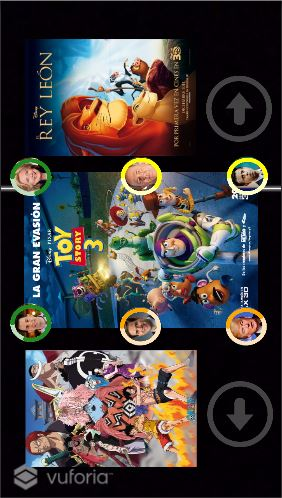
\includegraphics[width=3in, angle=270]{figures/chapter-2/recomendadorAR.JPG}
        \caption{Vista encargada de recomendar planes en RA al enfocar a un amigo}
\end{figure}
\begin{flushleft}
Como se puede ver en la figura 3.20, en la interfaz aparecen las tres películas, únicamente se muestra la 
información relacionada con los usuarios del plan situado en medio para no saturar la interfaz. Mediante los 
botones de izquierda y derecha el usuario puede moverse entre planes para poder ver la información necesaria 
de cada plan y elegir aquel que más le guste.
\end{flushleft}
\begin{flushleft}
La información visual que aparece relacionada con los usuarios representa:
\begin{itemize}
    \item Arriba a la izquierda el amigo que se encuentra ya en el plan junto con una representación gráfica 
    de cuanto estima el algoritmo de recomendación que le puede gustar la película.
    \item Arriba a la derecha, la foto del usuario que está valorando unirse al plan junto con una representación 
    gráfica de cuanto estima el algoritmo de recomendación que le puede gustar la película.
    \item El resto de las posiciones identifican al resto de usuarios junto con la representación gráfica de 
    cuanto se estima que le puede gustar la película.
    
\end{itemize}
\end{flushleft}

\subsection{Interfaz de inicio de sesión y de registro}
\label{makereference3.4.6}

Nos aparecerá una interfaz muy simple para realizar el inicio de sesión con un usuario en la aplicación al entrar. También nos permite registrarnos como usuarios si
aún no poseemos una cuenta en la aplicación.

\begin{figure}[H]
    \centering
    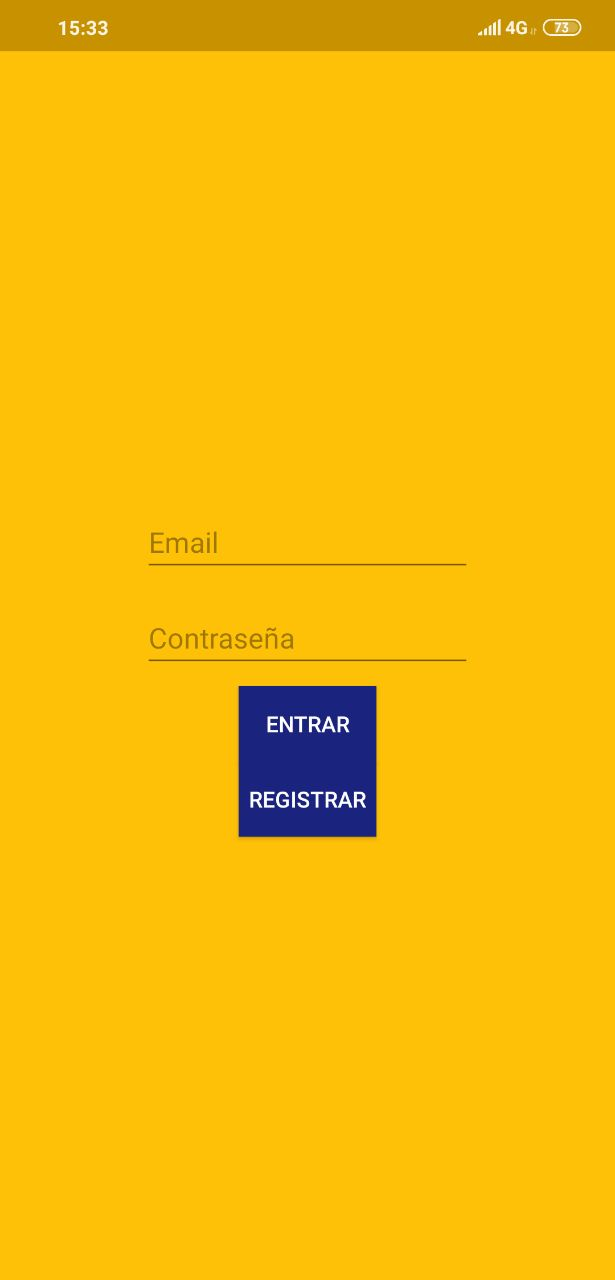
\includegraphics[height=4in]{figures/login.jpg}
    \caption{Inicio de sesión}
\end{figure}
\begin{figure}[H]
    \centering
    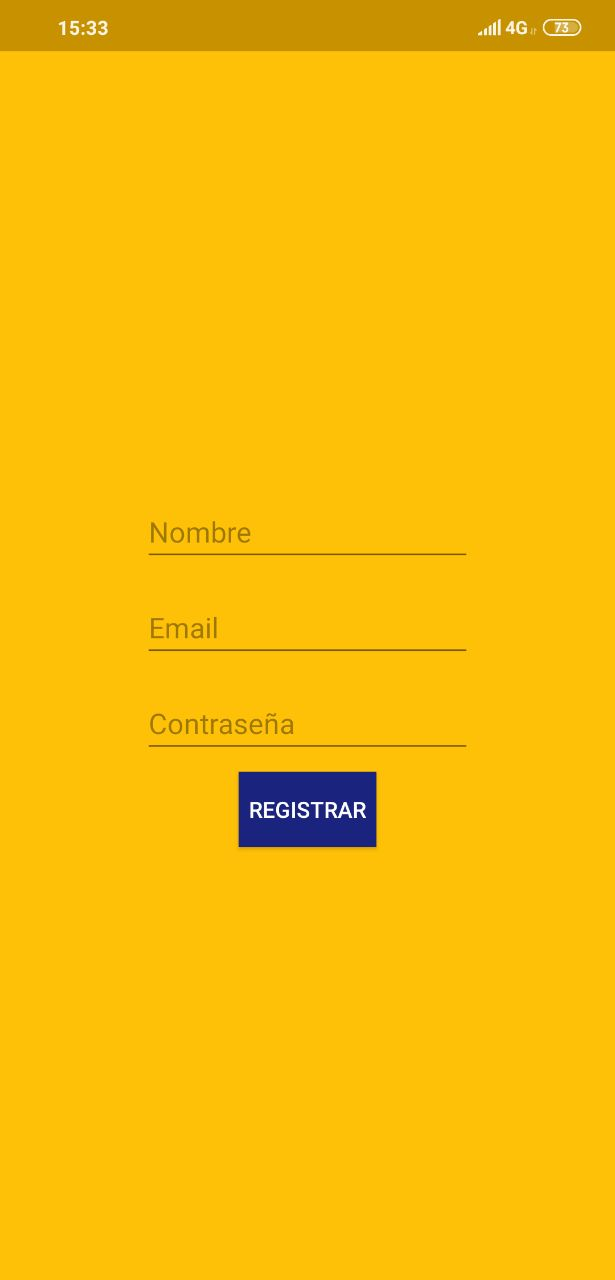
\includegraphics[height=4in]{figures/register.jpg}
    \caption{Registro}
\end{figure}

\subsection{Interfaz de recomendaciones}
\label{makereference3.4.7}

\subsection{Interfaz de información de una película}
\label{makereference3.4.8}

Tras pulsar en una de las películas que hemos guardado nos aparecerá dicha interfaz. 
Esta vista nos permite ver en primer plano el cartel de la película y la información correspondiente a la misma, como puede
ser la sinopsis de la película, el género y el nombre del director. Además, poseemos un \textbf{Gauge} que nos permite, al pulsarlo,
valorar la película mediante una barra de progreso.
Si hacemos scroll hacia abajo, la imagen de la película se irá ocultando para ofrecernos una mejor visión de la información de la película.
En la parte inferior se nos presentan dos botones, uno para crear un plan con la película, que es el de color amarillo con el texto: \textbf{AÑADIR AL PLAN}. El otro botón de color
violeta con el símbolo de reproducir un vídeo, nos llevará al trailer de la película en \textbf{Youtube}.
Arriba a la derecha observamos el icono de un corazón, lo que nos permitirá quitar esta película de nuestras favoritas y ya no aparecerá en la
lista de películas guardadas.

\begin{figure}[H]
    \centering
    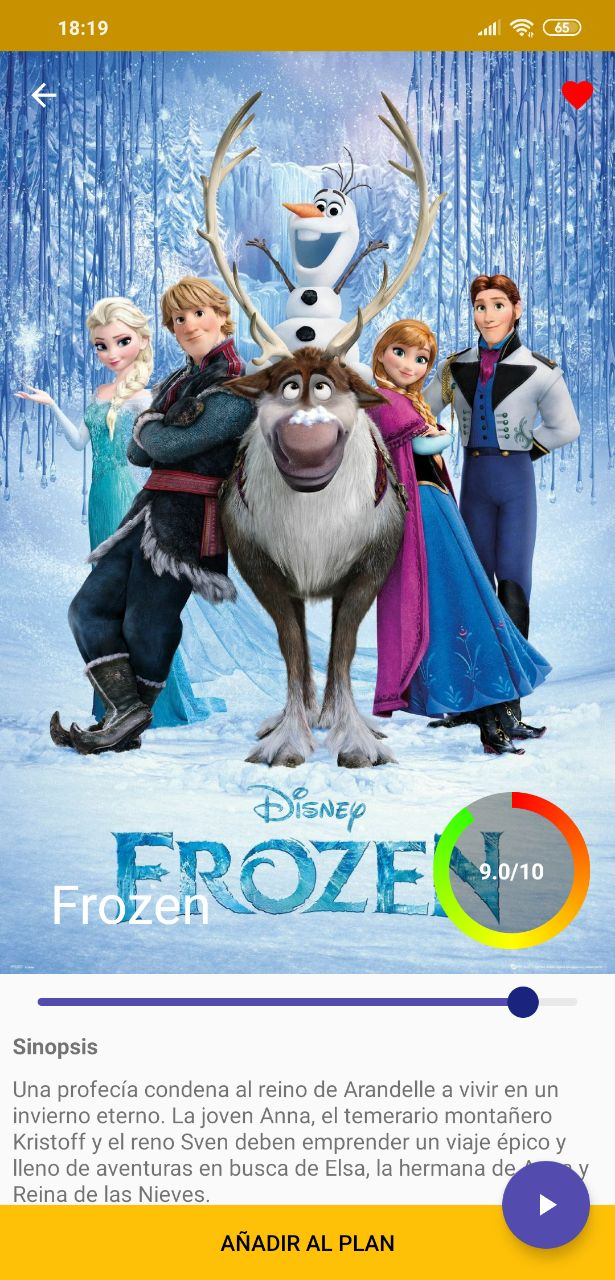
\includegraphics[width=3in]{figures/infoFilm1.jpg}
    \caption{Información de la película}
\end{figure}
\begin{figure}[H]
    \centering
    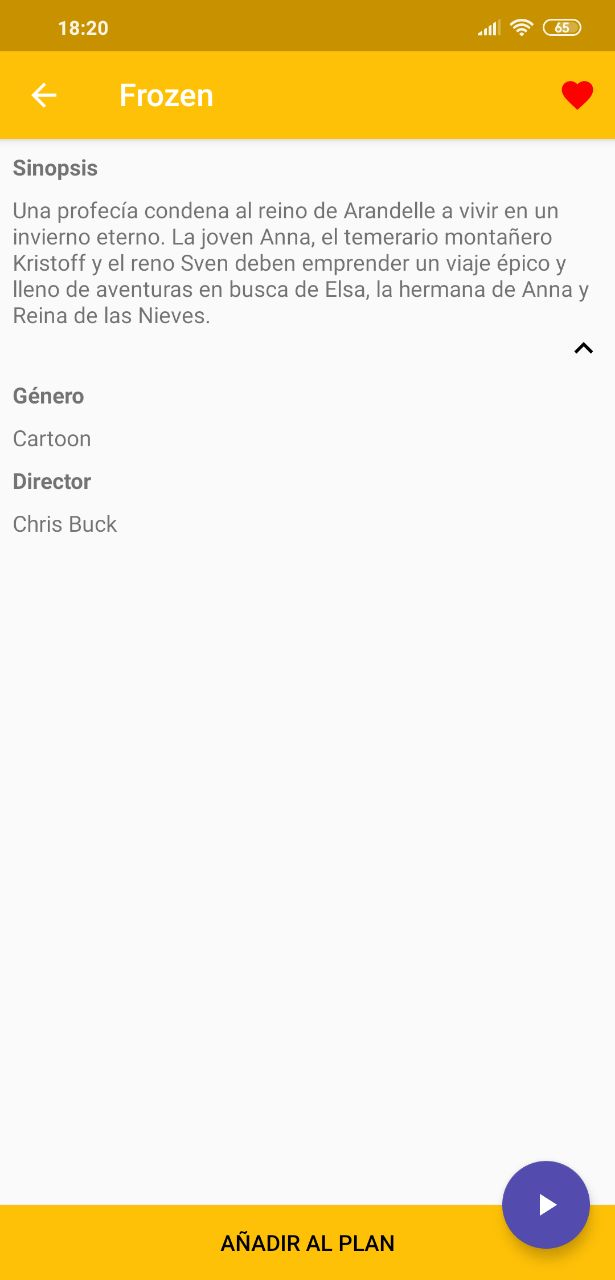
\includegraphics[width=3in]{figures/infoFilm2.jpg}
    \caption{Información de la película observando el cambio en el Gauge tras valorar}
\end{figure}
\begin{figure}[H]
    \centering
    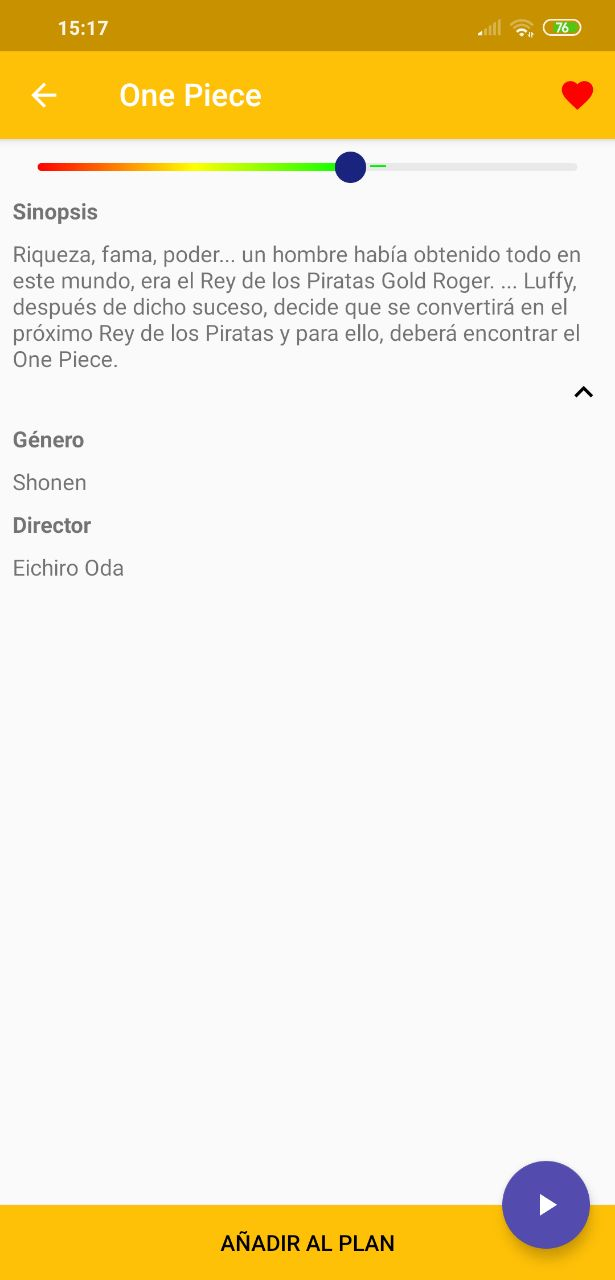
\includegraphics[width=3in]{figures/infoFilm3.jpg}
    \caption{Información de la película cuando se hace el scroll hacia abajo}
\end{figure}

\subsection{Interfaz de información de un plan}
\label{makereference3.4.9}
Esta interfaz aparece cuando pulsamos en un plan y es muy similar a la que se le muestra al usuario con la información
de una película. También nos aparecerá en grande la imagen de la película que se quiere ir a ver con dicho plan, junto con información
relevante de dicho plan, como puede ser:
\begin{itemize}
    \item \textbf{Fecha}: día, mes y año en el que tendrá lugar dicho plan.
    \item \textbf{Hora}: hora del plan.
    \item \textbf{Lugar}: localización que haya puesto el creador del plan para ver la película.
    \item \textbf{Descripción}: breves anotaciones características que haya escrito el creador sobre el plan.
    \item \textbf{Usuarios unidos}: imágenes de los usuarios que se han unido al plan.
\end{itemize}
Además, nos aparece un botón en la parte inferior con el texto: \textbf{UNIRSE AL PLAN} o \textbf{SALIR DEL PLAN}, según estemos o no ya dentro del plan.
También en la parte inferior derecha de la imagen de la película tenemos un botón que nos redirige a la interfaz de información de dicha película.
En la parte superior derecha nos aparece un icono de una basura, lo que nos permitirá borrar el plan, si somos el creador.
\begin{figure}[H]
    \centering
    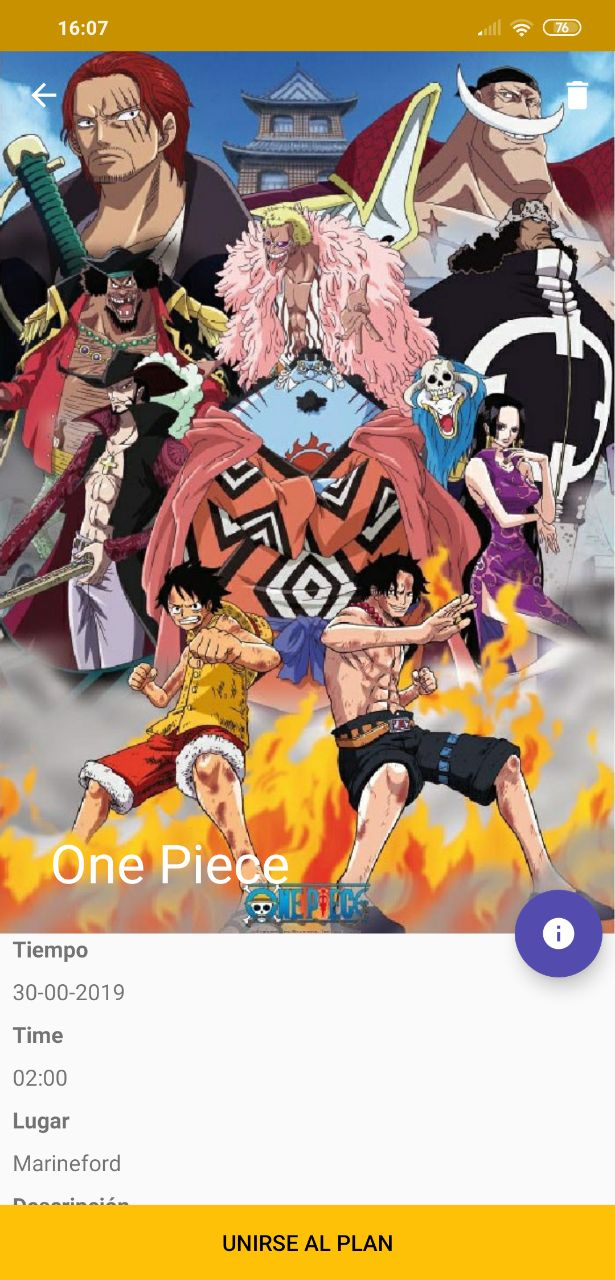
\includegraphics[width=3in]{figures/infoPlan1.jpg}
    \caption{Información del plan}
\end{figure}
\begin{figure}[H]
    \centering
    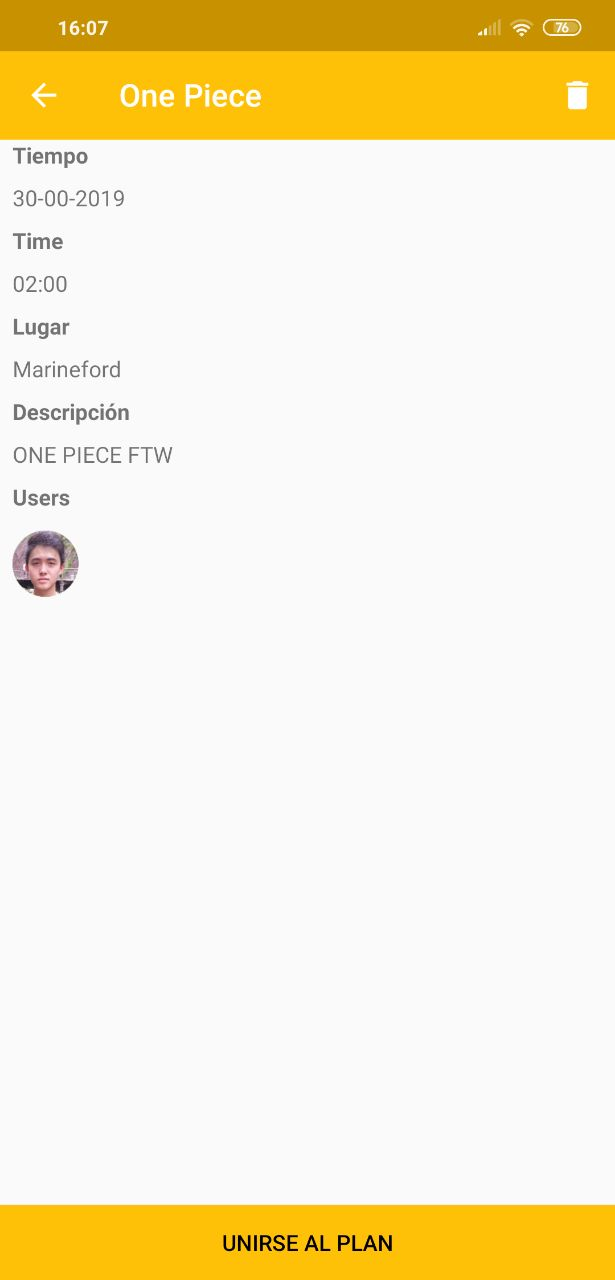
\includegraphics[width=3in]{figures/infoPlan2.jpg}
    \caption{Información del plan tras hacer el scroll hacia abajo}
\end{figure}